\documentclass[reprint,amsmath,amssymb,aps]{revtex4-2}%
\usepackage{unicode-math}
\usepackage{lmodern}%
\usepackage{textcomp}%
\usepackage{lastpage}%
\usepackage{graphicx}%
\usepackage{siunitx}%
%
%
\begin{document}%
\normalsize%
\title{Improving Nb\textsubscript{3}Sn Cavity Performance Using Centrifugal Barrel Polishing}%
\author{Eric Viklund}%
\email{ericviklund2023@u.northwestern.edu}
\affiliation{Department of Materials Science and Engineering, Northwestern University}%
\affiliation{Fermi National Accelerator Laboratory}%
\author{David N. Seidman}%
\affiliation{Department of Materials Science and Engineering, Northwestern University}%
\author{David Burk}%
\affiliation{Fermi National Accelerator Laboratory}%
\author{Sam Posen}%
\email{sposen@fnal.gov}
\affiliation{Fermi National Accelerator Laboratory}%
\date{\today}%

\begin{abstract}%
In this study we will show a new method of polishing for Nb\textsubscript{3}Sn cavities known as centrifugal barrel polishing (CBP). Using this method, Nb\textsubscript{3}Sn coated samples are polished to a surface roughness comparable to a traditional Nb cavity after electropolishing (EP). We also investigate different methods of cleaning the Nb\textsubscript{3}Sn surface after CBP to remove residual abrasive particles. The polished Nb\textsubscript{3}Sn surface is analyzed using confocal laser microscopy, and scanning electron microscopy (SEM) is used to image the surface and measure the surface roughness after polishing. Transmission electron microscopy (TEM) is also used for high resolution analysis of the surface after polishing. Finally, we show that centrifugal barrel polishing can improve the performance of a Nb\textsubscript{3}Sn SRF cavity.
%
\end{abstract}%

\maketitle%

\section{Introduction}%
\label{sec:Introduction}%
Superconducting radiofrequency (SRF) cavities are an essential component of particle accelerators used in various fields of science and industry, including high-energy physics, material science, and medical isotope production\cite{boulware2019high}. These cavities accelerate charged particles to very high energies and can achieve higher accelerating gradients at continuous operation than normal conducting cavities.

The performance of superconducting radio-frequency cavities is determined by the superconducting properties of the surface layer of the cavity. The low-temperature superconductor Nb\textsubscript{3}Sn has a higher superconducting transition temperature (T\textsubscript{c}), 18~K compared to 9~K, and a higher super-heating magnetic field (H\textsubscript{sh}), around 440~mT compared to 250~mT for the more commonly used niobium\cite{liarte2017theoretical, catelani2008temperature, lin2012effect, kubo2020superfluid}. SRF cavities coated with a layer of Nb\textsubscript{3}Sn can, therefore, achieve a much higher accelerating field, up to 100~MV/m in theory, and have a lower surface resistance than Nb SRF cavities at higher temperatures allowing for cavity operation at 4~K. Whereas Nb cavities are typically operated at 2~K e.g. the LCLS-II cryomodules\cite{galayda2018lcls}. These properties make Nb\textsubscript{3}Sn SRF cavities a promising research topic for future accelerators such as high-energy linacs or small-scale industrial accelerators.

Nb\textsubscript{3}Sn cavities are typically manufactured by coating a Nb cavity with a thin film of Nb\textsubscript{3}Sn using Sn vapor-diffusion\cite{posen2017nb3sn, pudasaini2019growth, porter2018update}, exposing a Nb cavity to tin vapor at 1,100~°C to create Nb\textsubscript{3}Sn. The reaction forms a 2-3~µm thick Nb\textsubscript{3}Sn film with grains approximately 1~\unit{\micro\metre} large. The grains are faceted, and the grain boundaries are thermally etched resulting in approximately 100-150~nm of surface roughness. 

Using the Sn vapor-diffusion coating technique\cite{posen2017nb3sn,pudasaini2019growth,eremeev2013development}, Nb\textsubscript{3}Sn cavities have only been able to reach a maximum accelerating gradient of 24~MV/m\cite{posen2021advances}, a result that was achieved using a thinner Nb\textsubscript{3}Sn coating which is smoother than the typical coating. However, this result has not been reproducible, and the performance is lower than the theoretical maximum of Nb\textsubscript{3}Sn cavities.

Surface roughness is thought to be one of the limiting factors of Nb\textsubscript{3}Sn SRF cavity performance. Surface roughness has been shown to be a cause of Q slope and quench in niobium cavities treated with buffered chemical polishing (BCP) due to sharp grain boundary steps.\cite{knobloch1999high, xu2016simulation} Simulations of the magnetic field near a typical Nb\textsubscript{3}Sn surface show that the magnetic field is increased by up to 60~percent in some areas compared to a smooth surface\cite{porter2016surface, kubo2015magnetic} and could be higher for particularly rough areas. By reducing the field enhancement caused by surface roughness, a corresponding increase in the cavity accelerating gradient can be expected. 

One method to achieve smoother Nb\textsubscript{3}Sn surfaces is polishing. Nb\textsubscript{3}Sn polishing has been a topic of study for some time. Chemical methods such as electropolishing (EP)\cite{pudasaini2018studies,pudasaini2017post,hu2019reducing}, buffered chemical polishing (BCP)\cite{pudasaini2017post,hu2019reducing}, and oxy-polishing\cite{pudasaini2017post,pudasaini2018studies} have been studied, but have failed to produce any meaningful improvement in surface roughness. The expected reason for this is that a large amount of material removal is required to produce a substantial smoothing effect when utilizing chemical methods. Electropolishing treatments for Nb typically remove between 5~µm and 10~µm of material to achieve a smooth surface depending on its initial roughness. This amount of material removal is infeasible for Nb\textsubscript{3}Sn films, since their thickness is only 2-3~µm. Additionally, niobium and Sn react differently to the chemicals used, which can lead to different removal rates for each element, thus changing the surface stoichiometry. Even a small change in the stoichiometry away from Nb\textsubscript{3}Sn can cause a decrease in T\textsubscript{c}\cite{sitaraman2021effect}.

To circumvent these issues, we instead use a technique known as centrifugal barrel polishing (CBP), a procedure commonly used for mechanically polishing Nb SRF cavities, and apply it to Nb\textsubscript{3}Sn cavities. First, Nb\textsubscript{3}Sn coated samples are polished to determine the effectiveness of the CBP method and to determine the optimum polishing parameters such as tumbling duration and the abrasive material. The results of the sample experiments are used to decide the polishing parameters for a Nb\textsubscript{3}Sn coated, 1.3~GHz, TESLA geometry SRF cavity. The RF performance of the cavity is tested before and after the CBP treatment. Finally, the cavity is treated with a low temperature Sn coating process to repair the surface and the RF performance is once again tested.

%
\section{sample study}%
\label{sec:samplestudy}%
Since Nb\textsubscript{3}Sn is a relatively unexplored material, there are no established polishing parameters or abrasive materials to achieve a good surface finish. To allow for rapid iteration and microscopy surface analysis, we first perform polishing experiments on Nb\textsubscript{3}Sn samples. To evaluate the performance of CBP, the surface roughness of the polished samples is measured using confocal laser microscopy and the surface is analyzed using scanning and transmission electron microscopy (SEM and TEM). The material removal rate is measured using focused ion-beam tomography.

The samples were prepared using the standard Nb\textsubscript{3}Sn coating procedure. 1~\unit{\centi\metre} disks are cut from a 4~\unit{\milli\metre} sheet of fine-grain, low RRR niobium. 100~\unit{\micro\metre} of material are removed using standard electropolishing\cite{saito2003development}, followed by 5~\unit{\micro\metre} of removal using cold EP leading to a root-mean-square surface roughness of 20~nm for the initial substrate.\cite{crawford2017extreme} The samples are coated with the standard FNAL coating procedure.\cite{posen2017nb3sn} This coating resulted in an approximately 3~\unit{\micro\metre} thick film with a grain size of 500~\unit{\nano\metre} and a surface roughness of 200~nm as shown in Fig.~\ref{fig:surfaceroughnessgraph}. The grain size of the Nb substrate had no effect on the film grain size.
%
\subsection{Centrifugal Barrel Polishing}% 
\label{subsec:CentrifugalBarrelPolishing}%
Centrifugal barrel polishing (CBP) is another method used to polish SRF cavities utilizing an abrasive material to mechanically smooth the surface. Tumbling was first implemented for SRF cavities by KEK and Nomura Plating Co. in 1995\cite{higuchi1996investigation}. This method has been used to repair surface damage and to attain a very smooth surface in Nb SRF cavities\cite{cooper2012mirror, cooper2011centrifugal}. 

As yet, only very limited attempts to apply this technique to Nb\textsubscript{3}Sn cavities have been made. The technique uses a custom-built tumbling machine that can fit up to 9-cell size 1.3~GHz cavities. When a cavity is mounted in the tumbling machine and filled with abrasive slurry, the rotating motion of the cavity accelerates the polishing media against the cavity surface at up to 59~\unit{\metre\per\square\second}. 

The abrasive material determines the removal rate and minimum surface roughness attainable using CBP. Large-grit material is used to remove material quickly and smooth out large defects like pits and scratches while fine-grit material is used to microscopically smooth the surface. Since the roughness of as-coated Nb\textsubscript{3}Sn cavities is on the order of 100-200~nm, our experiments focus on using fine-grit materials. In this experiment, we use a colloidal nanoparticle suspension, purchased from Allied High Tech Products Incorporated, as our abrasive material. 50~nm diameter alumina and 40~nm diameter silica nanoparticles suspended in water were tested, but we found no discernible difference between the polishing characteristics of the two materials.

Silicon containing ceramics, such as silica, are a major concern for contamination in the tin coating furnace, since they can release a significant amount of silicon at high temperatures into the furnace. Silicon also reacts with Nb\textsubscript{3}Sn to form poorly superconducting silicide phases. Alumina, in contrast, is thermally stable at higher temperatures. This is why alumina is typically used to electrically insulate wires such as thermocouples inside the furnace. For these reasons, the alumina abrasive particles are preferable to avoid any risk of furnace contamination.

The nanoparticle suspension was mixed with a large, soft material to act as a carrier. The purpose of the carrier material is to carry the nanoparticles and to apply a force between them and the cavity surface. Two carrier materials were tested, 13~mm diameter wooden balls and 25~mm compressed wool cubes supplied by Congress Tools, Incorporated.

%
\subsection{Coupon Cavity}%
\label{subsec:couponcavity}%
To test the centrifugal barrel polishing method on Nb\textsubscript{3}Sn samples in a realistic environment, we use a coupon cavity\cite{higuchi1996investigation}. This cavity has multiple ports where samples are mounted. The samples sit flush with the inside surface of the coupon cavity, as is shown in Fig.~\ref{fig:couponcavity}, where they experience identical polishing conditions to a real cavity surface. This allows for sample experiments that are representative of the final cavity polishing process. Using this method we inspect the Nb\textsubscript{3}Sn surface after polishing under a microscope to determine the best polishing parameters.

CBP was applied to samples mounted in the coupon cavity using the tumbling machine at FNAL. A total of four samples where polished for a duration of 2, 4, 6, and 8~\unit{\hour} respectively. The machine was run at its maximum speed of 120~RPM for the entire duration.
%


\begin{figure}[htb]%
\centering%
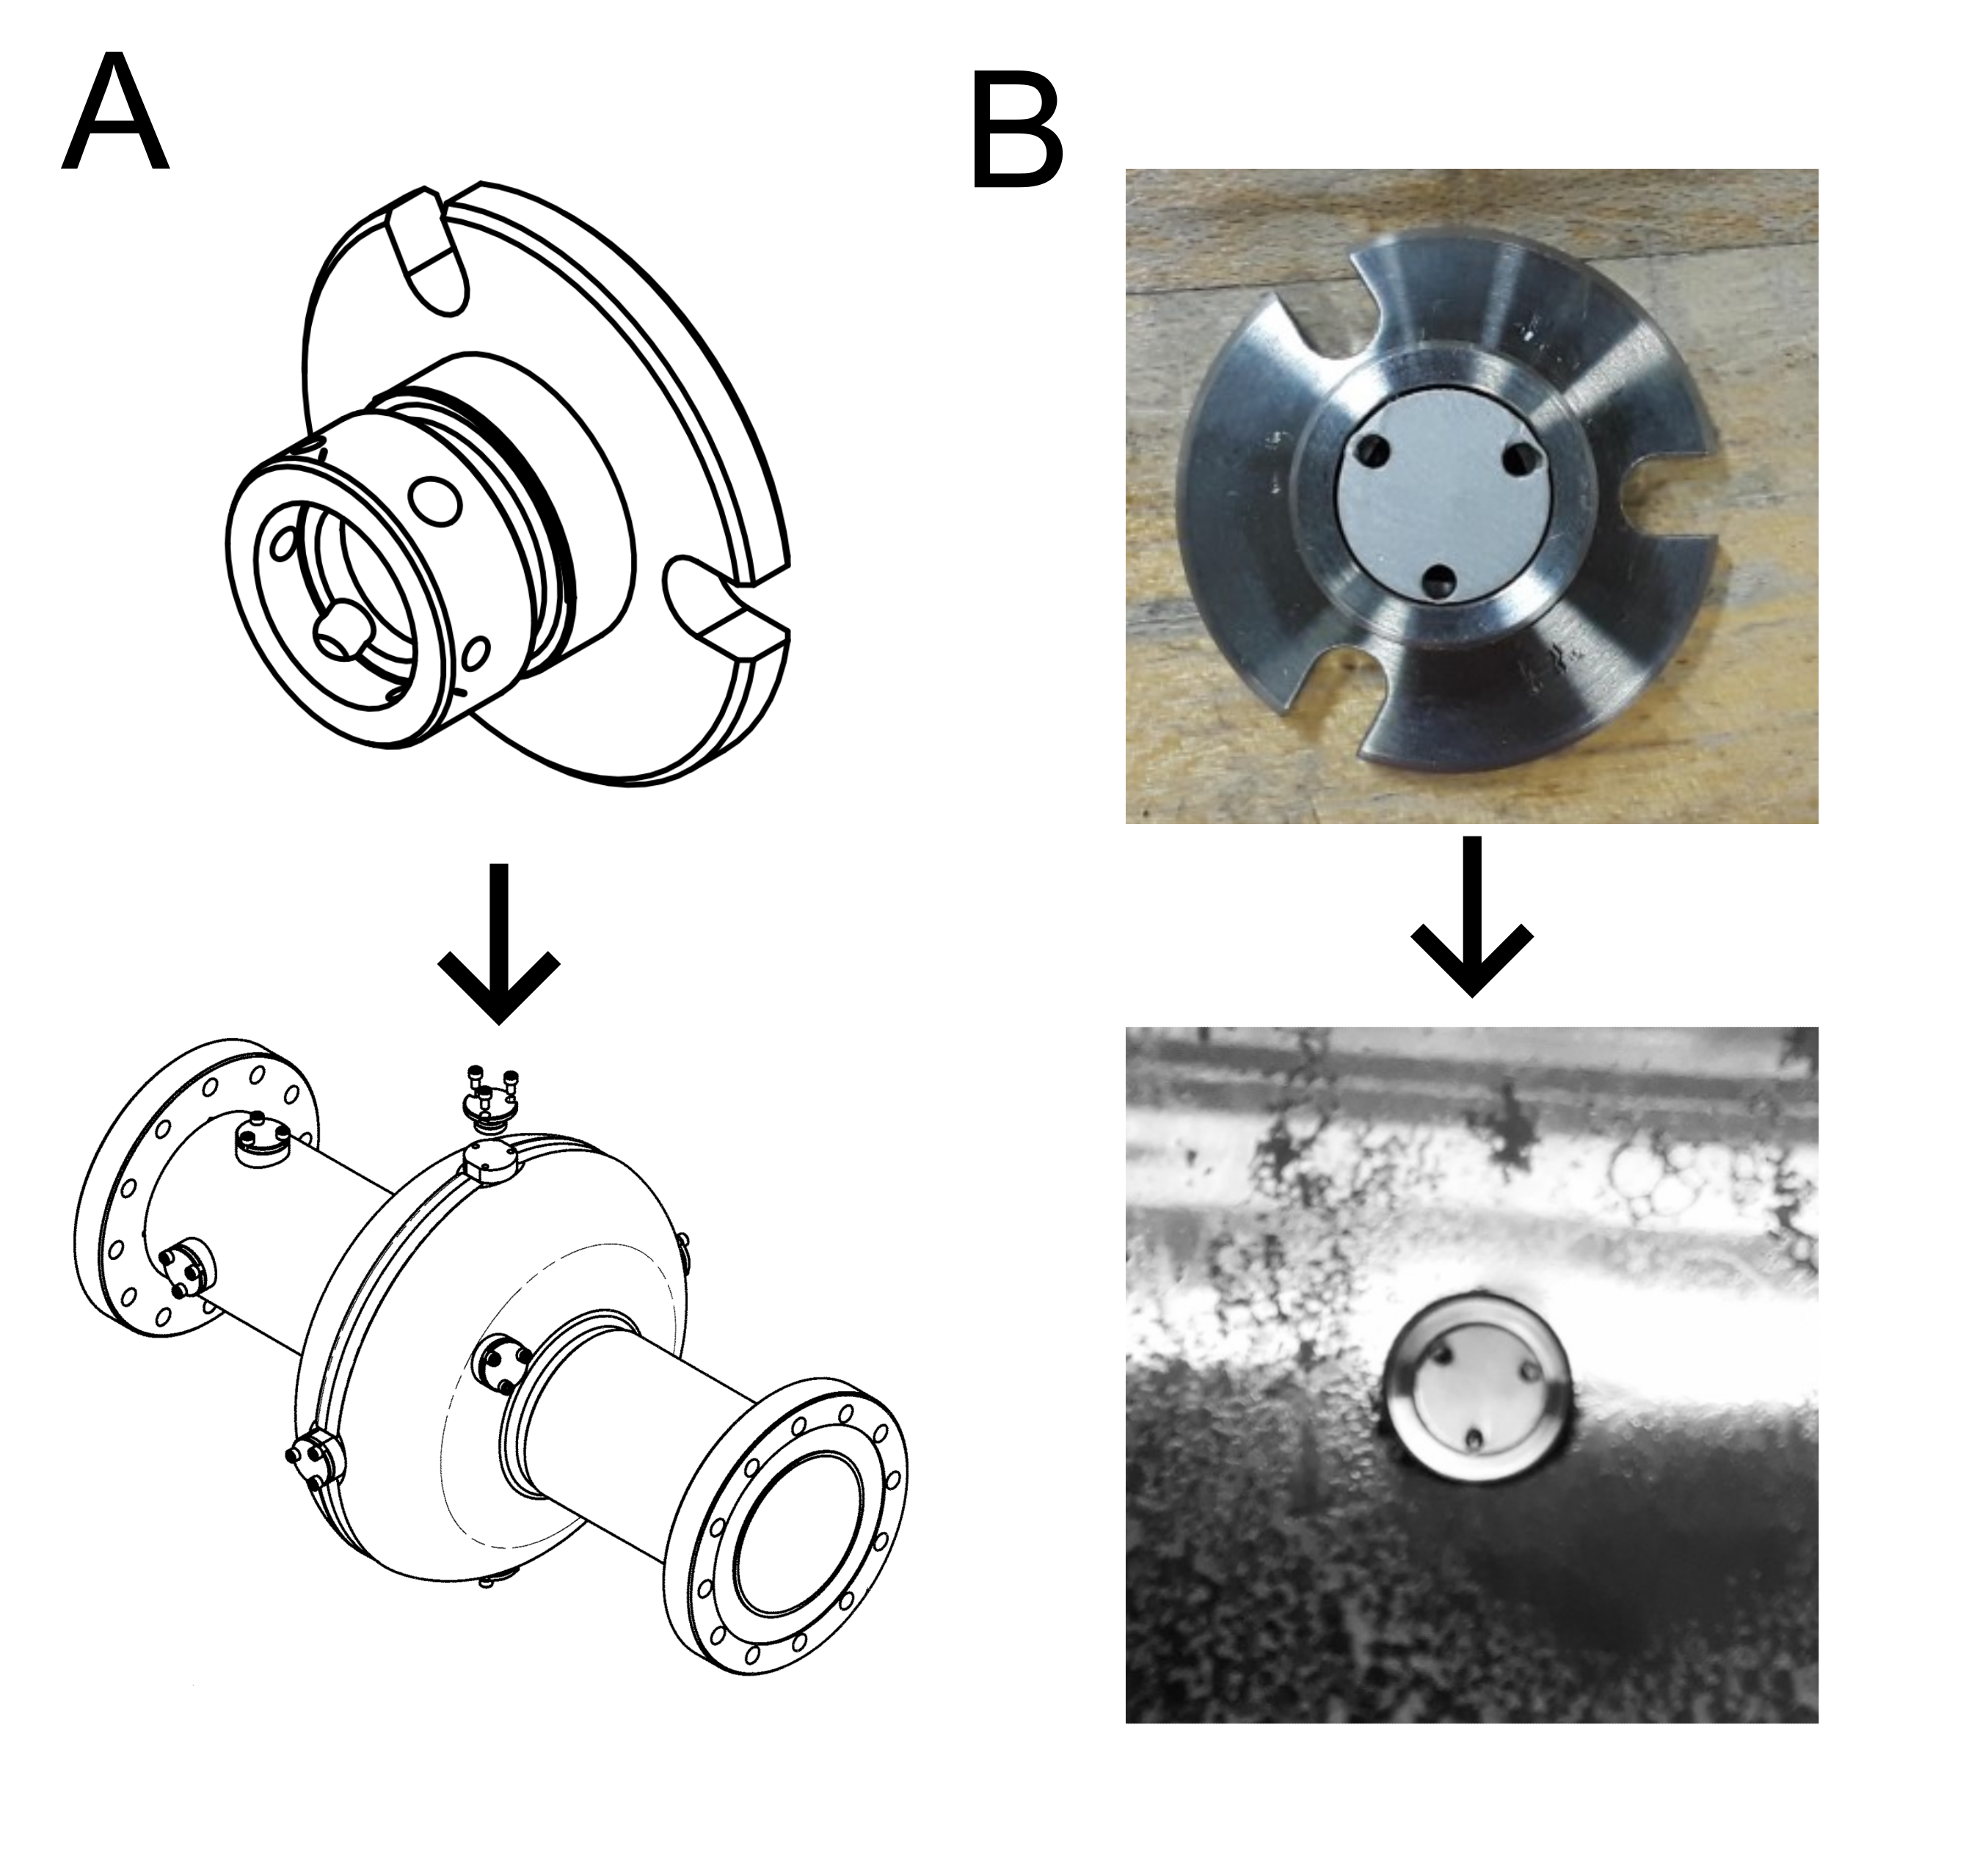
\includegraphics[width=\columnwidth]{../doc/figs/Coupon_Cavity.png}%
\caption{(A) A schematic of the coupon cavity and the sample holder used to polish the Nb\textsubscript{3}Sn coated samples. The sample holder can hold 1~cm diameter disks by clamping the sides of the sample with set screws. (B) Pictures of the sample holder sitting outside the coupon cavity with a sample mounted and as seen from the inside of the coupon cavity.}%
\label{fig:couponcavity}%
\end{figure}

%
\subsection{Nb\textsubscript{3}Sn Coating Using Sn Vapor-Diffusion}%
\label{subsec:nb3sncoating}%
The Nb\textsubscript{3}Sn samples used in this study were coated at Fermilab in a high-vacuum furnace. The coatings were created at 1,100~°C with a Sn crucible acting as the Sn source as well as SnCl\textsubscript{2} acting as a nucleating agent. A detailed review of the coating system at Fermilab shows the specific operating details of the coating system\cite{posen2017nb3sn}.

%
\subsection{Surface Analysis of Mechanically Polished Nb\textsubscript{3}Sn Coated Samples}%
\label{subsec:sampleanalysis}%
The Nb\textsubscript{3}Sn samples were polished for different lengths of time ranging from 2 to 8~hours using the wooden spheres or the felt cubes as the carrier material. Height maps of the polished samples measured using confocal laser microscopy is shown in Fig.~\ref{fig:opticalsurfaceprofiles}. The smoothness of the samples clearly improves as longer polishing is applied.

\begin{figure}[t]%
\centering%
\includegraphics[width=0.8\columnwidth]{../doc/figs/Optical_Surface_Profiles.png}%
\caption{Surface height maps of Nb\textsubscript{3}Sn samples mechanically polished for different lengths of time ranging from 2 to 8~hours compared to the initial state of the Nb\textsubscript{3}Sn coating. Measurements were performed with a Keyence VK-X3000 confocal laser microscope with a pixel size of 20~nm.}%
\label{fig:opticalsurfaceprofiles}%
\end{figure}

%


\begin{figure}[t]%
\centering%
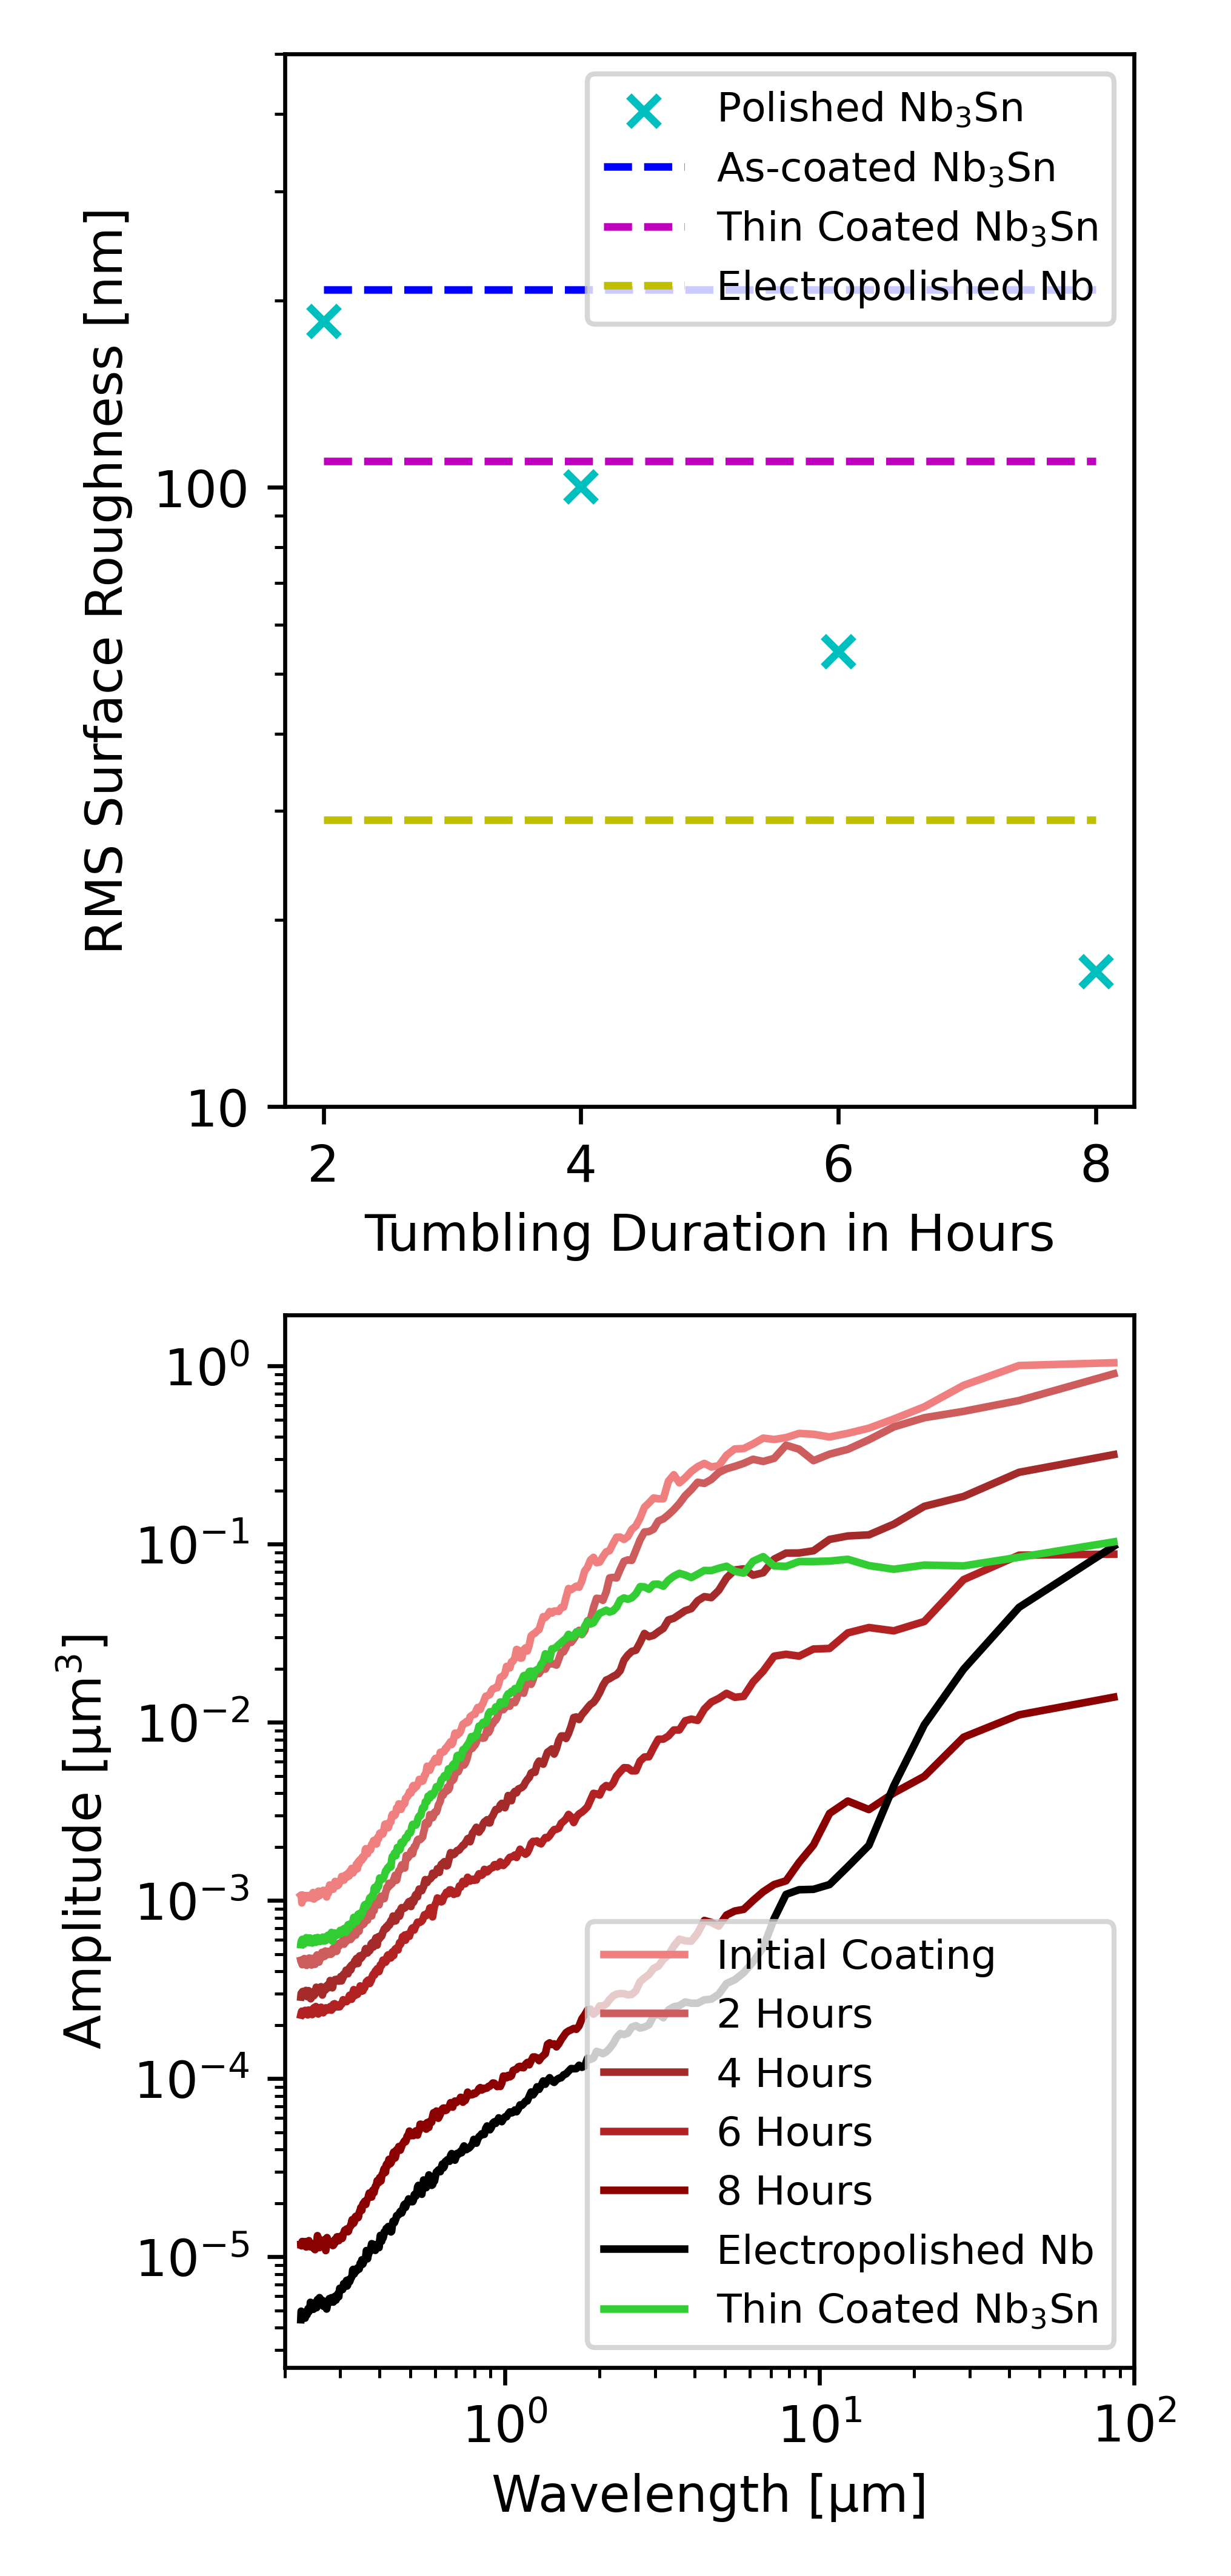
\includegraphics[width=0.8\columnwidth]{../doc/figs/Surface_Roughness_Graph.png}%
\caption{Surface roughness of Nb\textsubscript{3}Sn samples mechanically polished for different lengths of time calculated from the surface height maps (top). The power spectral density (PSD) of the surface profile after different amounts of tumbling as well as the PSD of electropolished Nb and a thinly coated Nb\textsubscript{3}Sn\ref{posen2021advances} film (bottom). The PSD is an indicator of the surface roughness of the sample at different length scales.}%
\label{fig:surfaceroughnessgraph}%
\end{figure}

%


\begin{figure}[t]%
\centering%
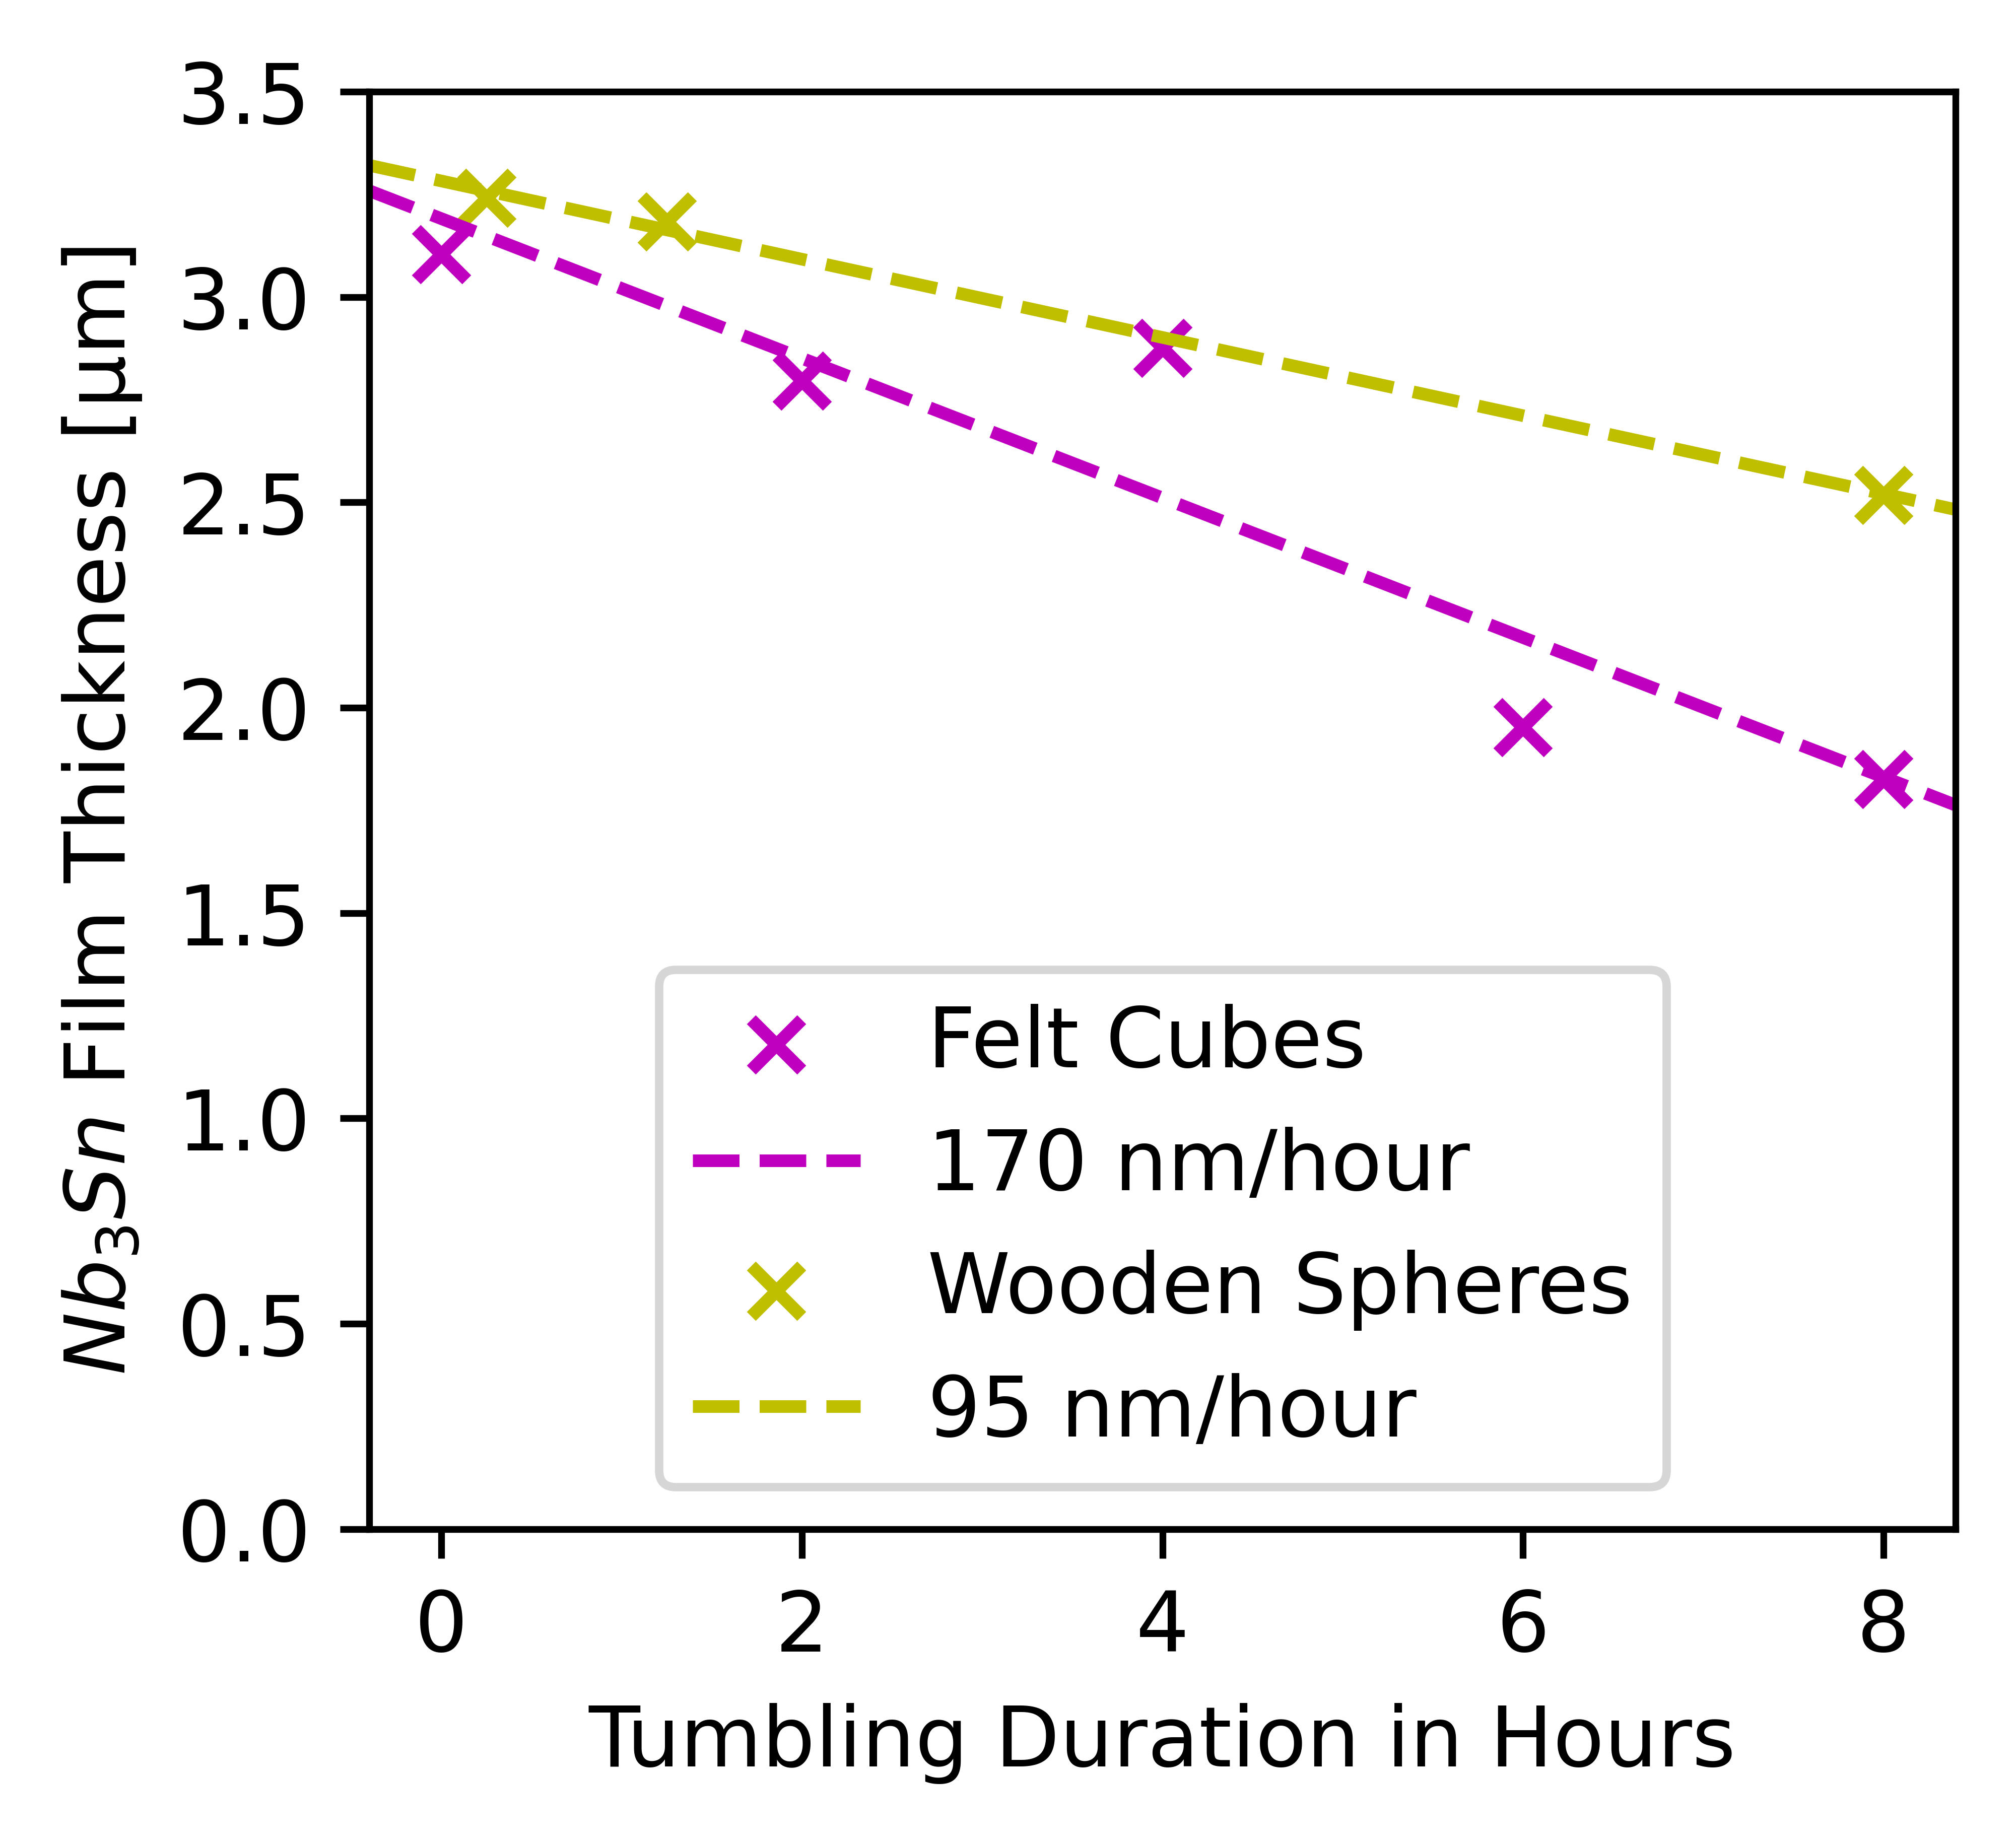
\includegraphics[width=0.8\columnwidth]{../doc/figs/Material_Removal_Graph.png}%
\caption{The thickness of the Nb\textsubscript{3}Sn film after mechanically polished for different lengths of time using felt cubes or wooden spheres as the polishing media.}%
\label{fig:materialremovalgraph}%
\end{figure}

By comparing the surface optical micrographs after different amounts of polishing shown in Fig.~\ref{fig:opticalsurfaceprofiles}, it is clear that material is preferentially removed from the highest point on the surface, causing the sharp peaks on the surface to be removed quickly while valleys are left untouched. The phenomenon is also clearly seen in SEM images of the samples shown in Fig.~\ref{fig:semimages} where the peaks on the grains can be seen to become smoother and then flat as more polishing is applied. This is different from EP, which preferentially smooths areas with high curvature including both peaks and valleys. Due to this different smoothing mechanism, surface roughness is minimized when the thickness of material removed is equal to the height difference between the highest and lowest point on the surface, which is around 1~µm. This is confirmed by the sample experiments, after 8~hours of polishing only the deepest valleys of the initial coating remain.

The surface height maps are used to calculate the root-mean-square (RMS) surface roughness of the samples and is shown in Fig.~\ref{fig:surfaceroughnessgraph}. After 6~hours of polishing the surface roughness is comparable to the surface roughness of the well performing, thinly coated Nb\textsubscript{3}Sn coatings created at FNAL\cite{posen2021advances}. We also calculate the power spectral density (PSD) of the surface profiles. The PSD is an indicator of the surface roughness at different length scales, indicated by the wavelength\cite{xu2011enhanced, pudasaini2017surface}.

This is verified by SEM micrographs of a thinly coated sample and a polished sample shown in Fig.~\ref{fig:semimages}A and D. After 8~hours of polishing, the surface roughness is comparable to a typical Nb surface after EP. This level of smoothness has never been achieved for Nb\textsubscript{3}Sn cavities until now. At this level of surface roughness, the performance degradation caused by field enhancement due to surface roughness should be greatly reduced.

The thickness of the film is measured after polishing using FIB/SEM cross-section measurements. Our measurements show that only a small amount of material is removed even after 8~hours of polishing. Fig.~\ref{fig:materialremovalgraph} shows the removal rate of different polishing materials. Samples polished using the felt media show an average removal rate of 170~nm/hour whereas the wooden media shows an average of 95~nm/hour removal rate. This measurement corresponds well with measurement performed on Nb cavities by Palczewski, Et. Al.\cite{palczewski2013exploration} The starting thickness of the samples is between 3-3.5~µm. After 8 hours of polishing there is still over 1.5~µm of Nb\textsubscript{3}Sn left on the surface. To completely shield the Nb substrate from the RF fields only a few hundred nanometers of material are required, since the London penetration depth of Nb\textsubscript{3}Sn is approximately 100~nm\cite{liarte2017theoretical}.

The surface of the polished samples was analyzed using SEM and TEM to look for surface damage or chemical changes on the surface caused by the tumbling or cleaning process. As seen in Fig.~\ref{fig:samplesurfacescratches} and Fig.~\ref{fig:samplesurfacedamagelayer}, the Nb\textsubscript{3}Sn samples polished using wooden spheres were damaged resulting in microscopic scratches on the surface and a nanometer-scale damaged layer. The damaged layer is theorized to consist of disordered Nb\textsubscript{3}Sn layer as no atomic layers are visible and attempts to rotate the sample to align the zone axis in this region were unsuccessful. No surface damage was detected on samples polished using the felt cubes. The surface and oxide layer of the sample polished with felt cubes looks similar to the as coated surface\cite{sun2023surface,cano2023selective}. Since the surface damage may negatively affect the cavity performance, the felt cubes are best to use for polishing Nb\textsubscript{3}Sn.
%




%


\begin{figure}[t]%
\centering%
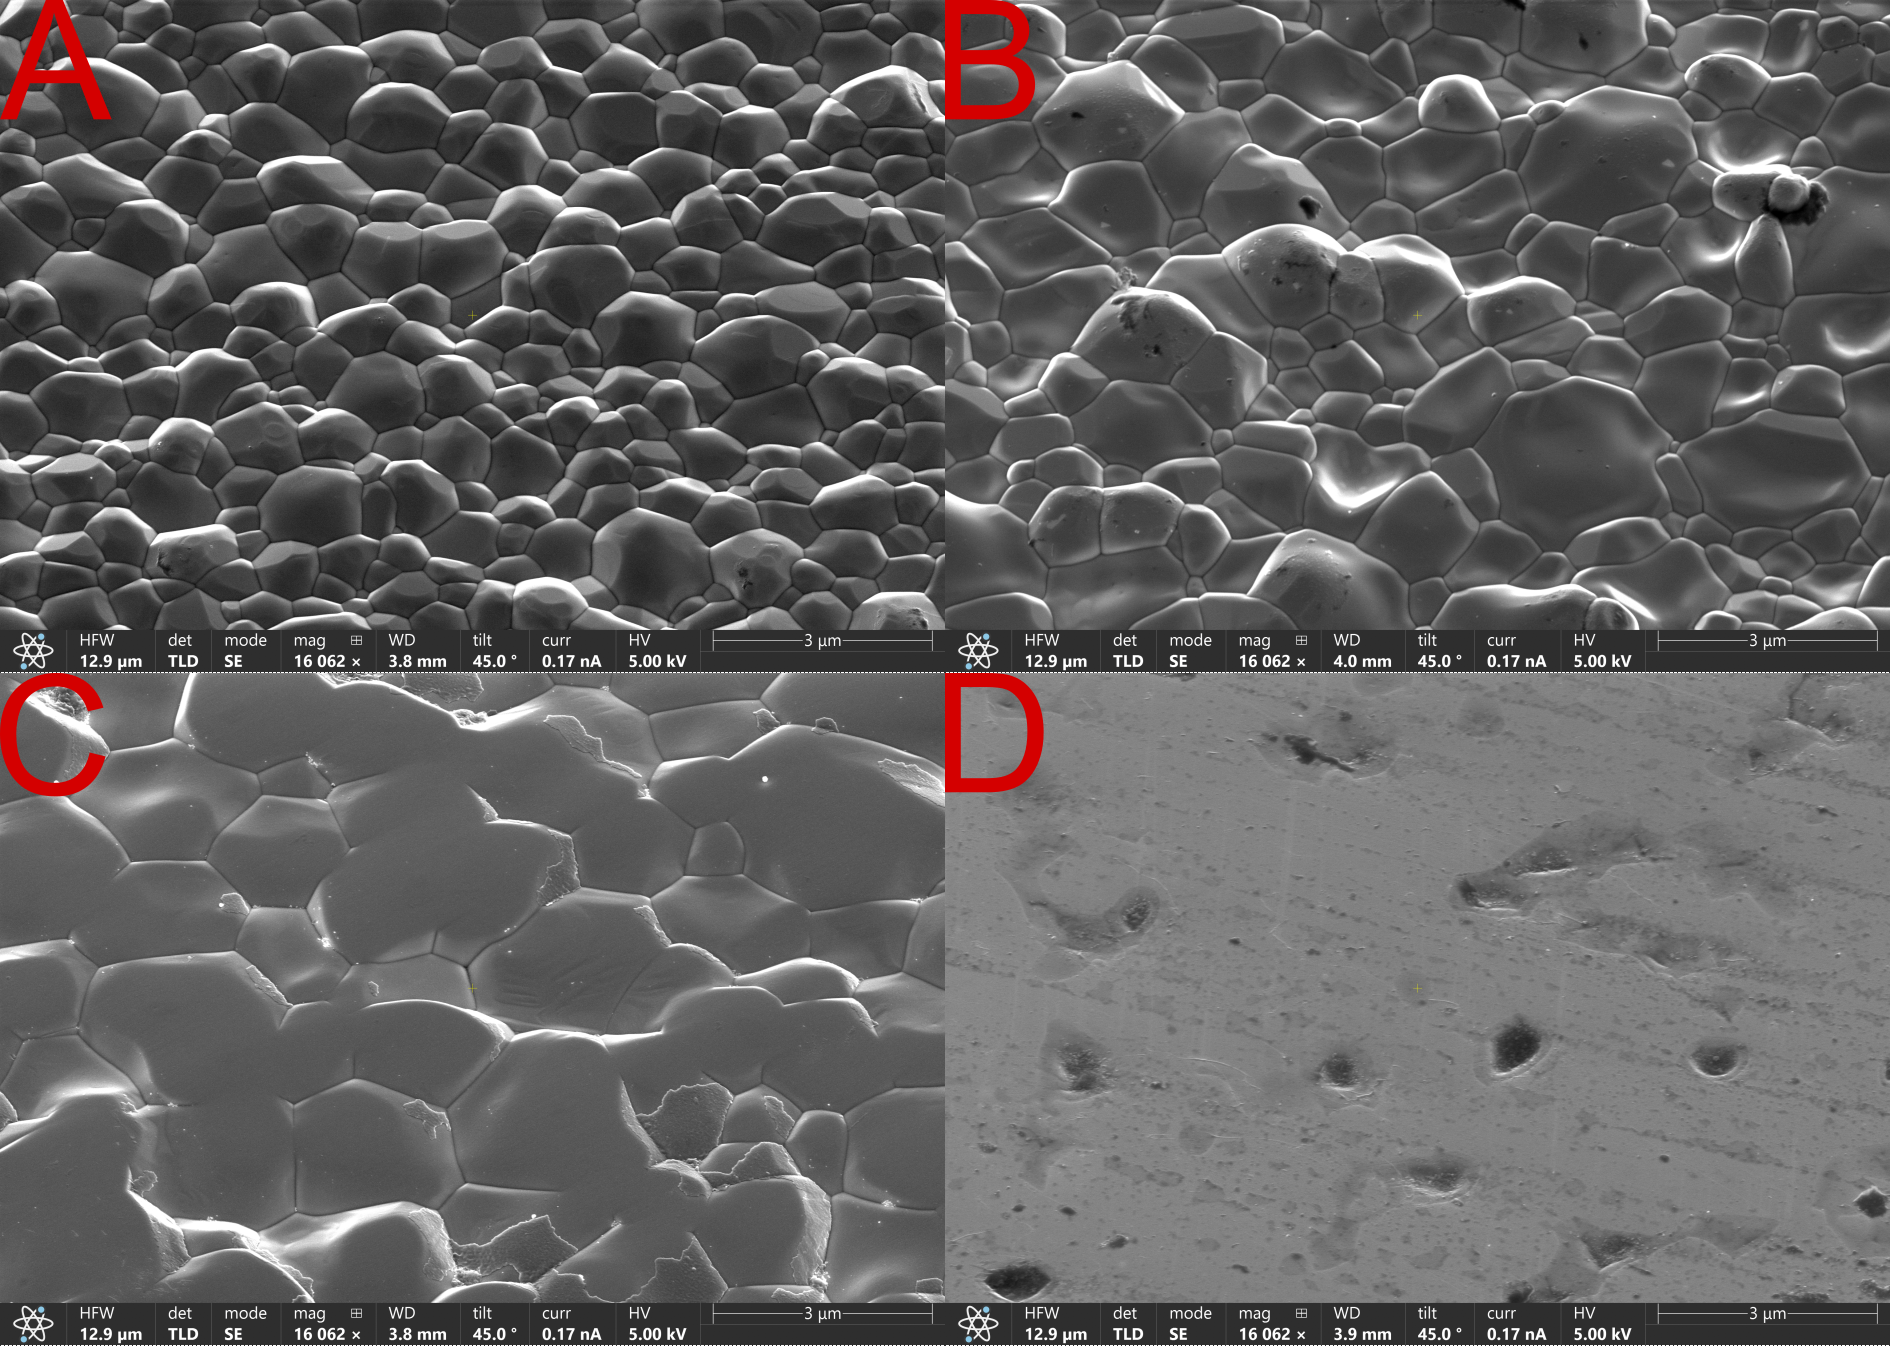
\includegraphics[width=0.8\columnwidth]{../doc/figs/SEM_Images.png}%
\caption{SEM micrographs of a Nb\textsubscript{3}Sn a thin coated sample (A), standard coated sample (B), a sample after polishing for 2~hours (C), and a sample after polishing for 6~hours (D).}%
\label{fig:semimages}%
\end{figure}

%


\begin{figure}[t]%
\centering%
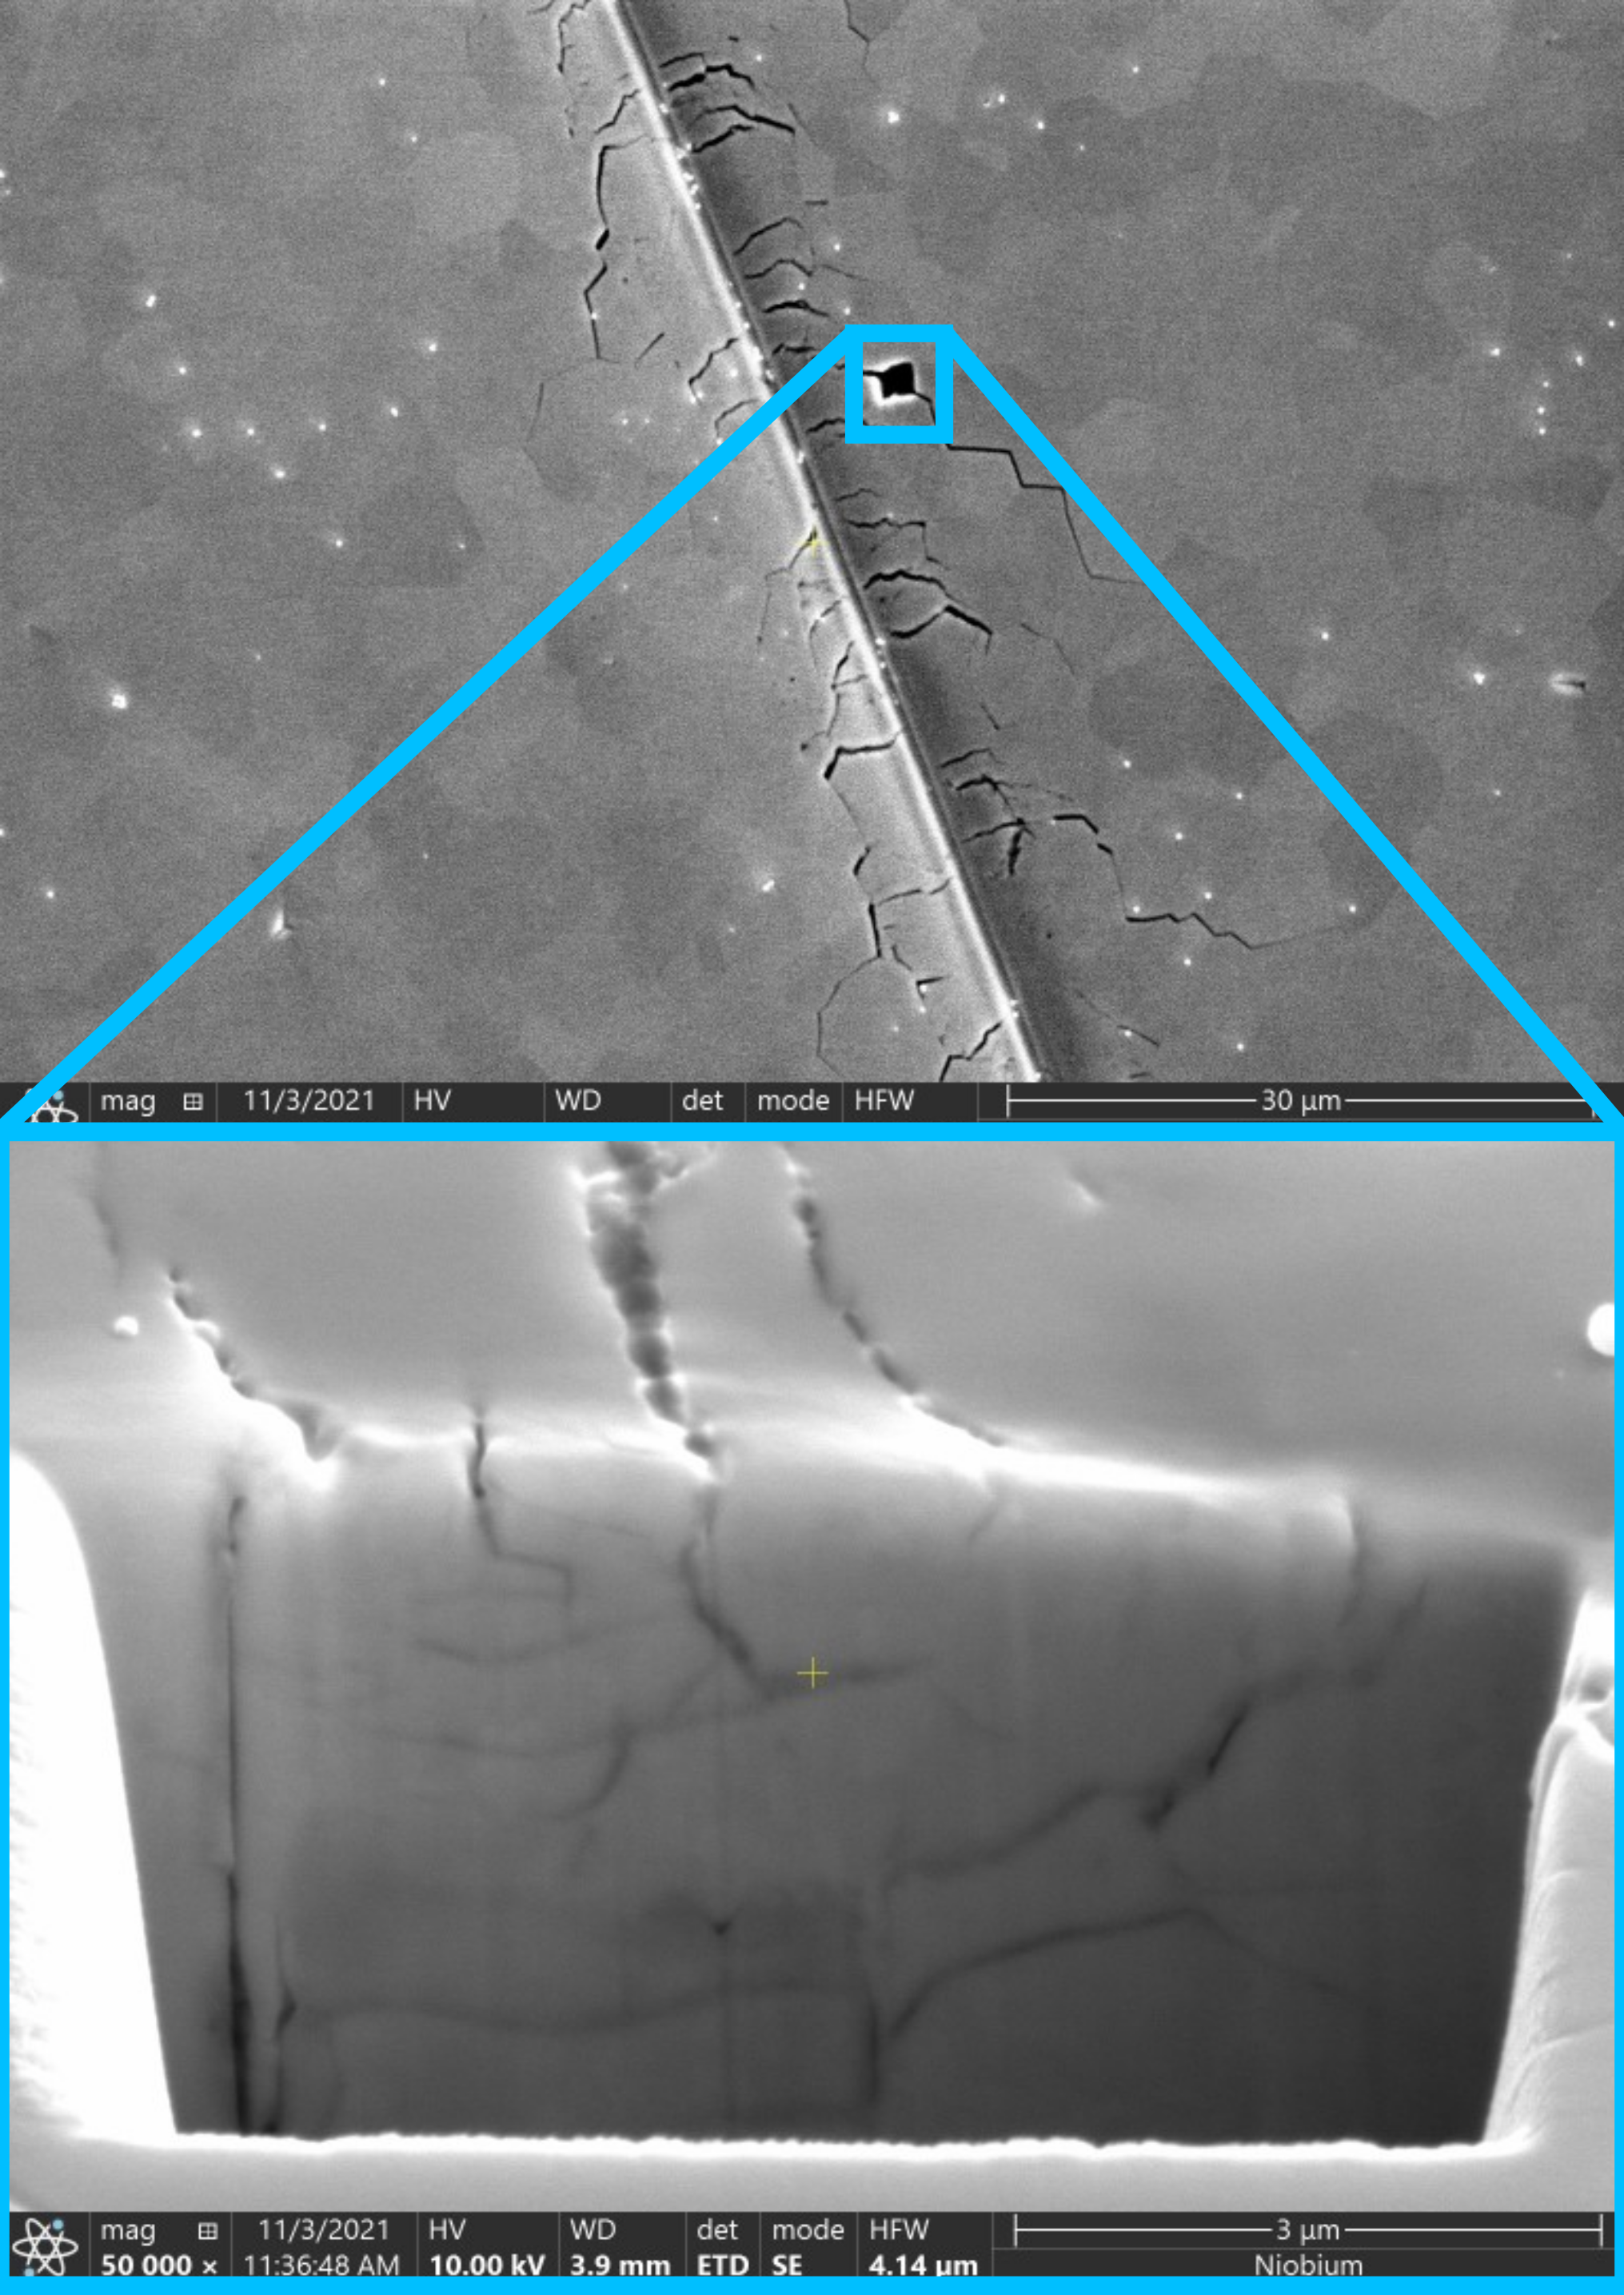
\includegraphics[width=0.8\columnwidth]{../doc/figs/Sample_Surface_Scratches.png}%
\caption{SEM micrograph showing a Nb\textsubscript{3}Sn sample polished for 30 hours using wooden spheres and a colloidal abrasive suspension. Nb\textsubscript{3}Sn films polished using wooden spheres show microscopic scratches and cracks on the surface. A square hole is cut into the surface, visible in the top micrograph to expose a cross-section of a crack. The cross-section shows that the cracks penetrate deep into the film.}%
\label{fig:samplesurfacescratches}%
\end{figure}

%


\begin{figure}[t]%
\centering%
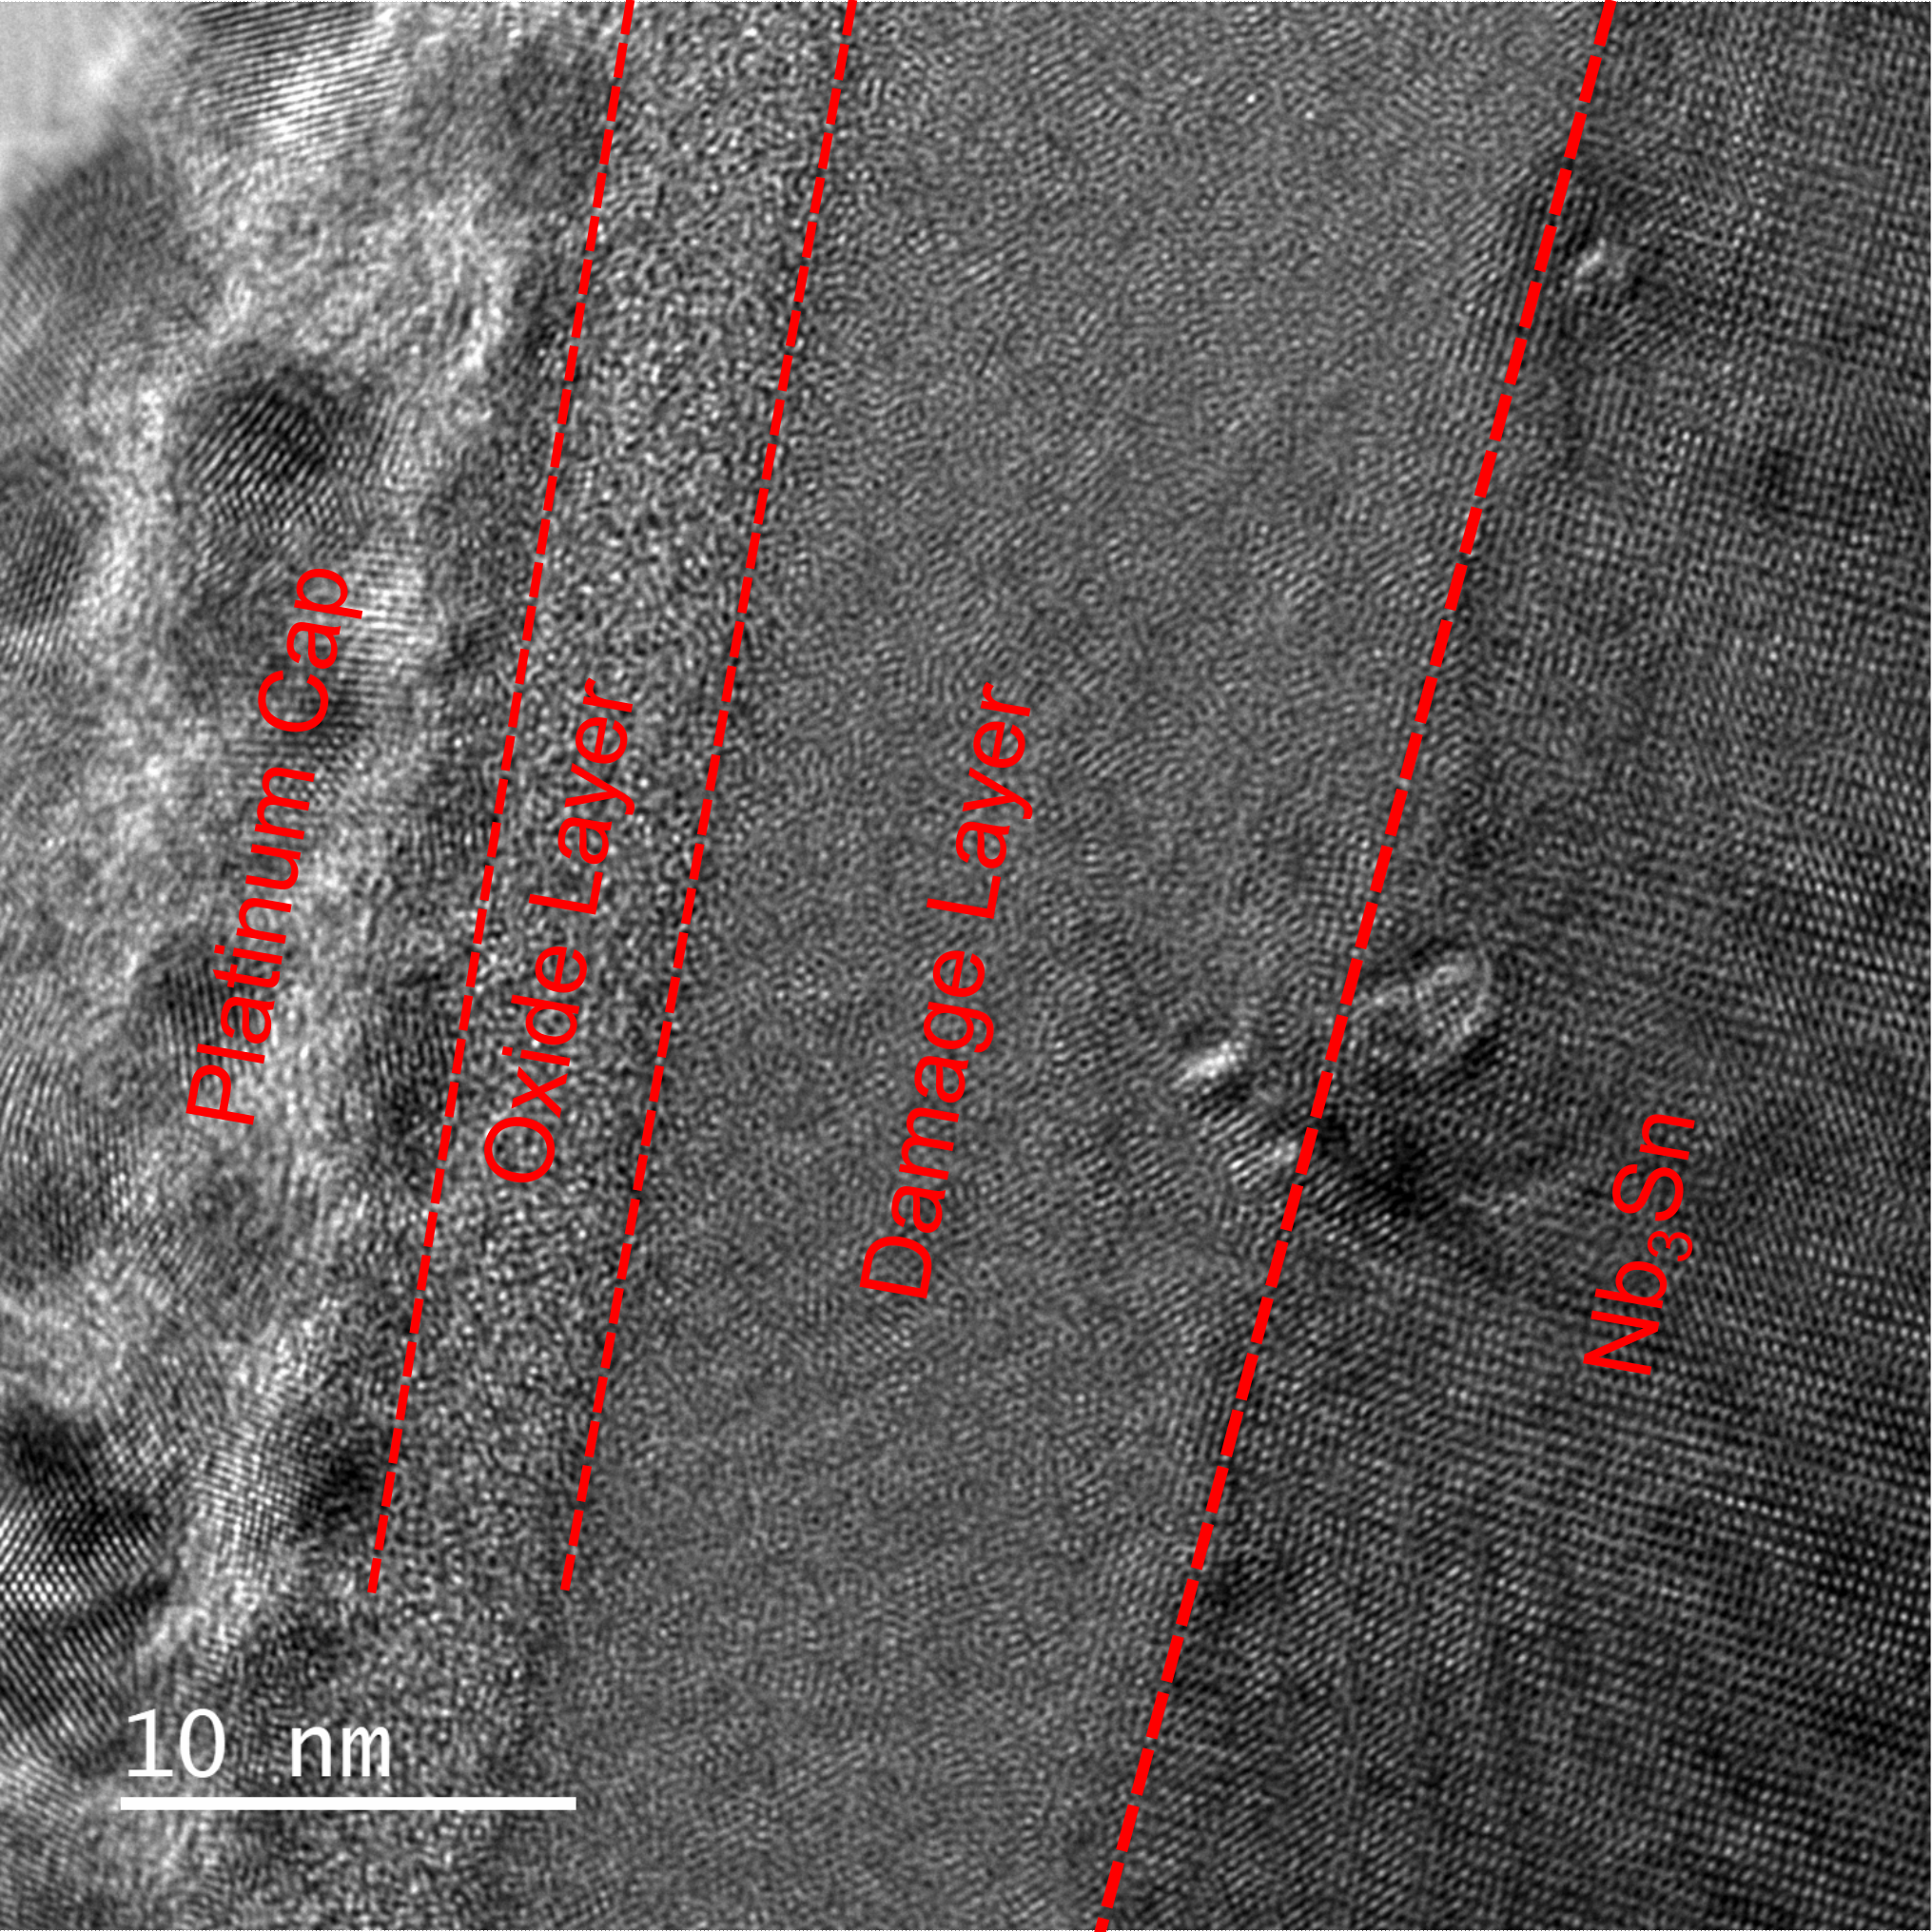
\includegraphics[width=0.8\columnwidth]{../doc/figs/Sample_Surface_Damage_Layer.png}%
\caption{TEM images of a Nb\textsubscript{3}Sn sample polished using wooden spheres (A) and felt cubes (B). The polishing procedure creates a 10~nm thick layer of disordered Nb\textsubscript{3}Sn, characterized by the absence of visible atomic planes and the clusters of dislocations on the interface with the ordered Nb\textsubscript{3}Sn, on the sample polished with wooden spheres which is not present on the sample polished by felt cubes.}%
\label{fig:samplesurfacedamagelayer}%
\end{figure}

%
\section{Polishing a Nb\textsubscript{3}Sn Cavity Using CBP}%
\label{sec:cavitycbp}%
Given that CBP was able to produce a smooth surface on Nb\textsubscript{3}Sn samples, the next step is to apply the polishing to a Nb\textsubscript{3}Sn cavity. The cavity used as the substrate for this experiment is a 1.3~GHz niobium elliptical cavity. The cavity is made of 2.8~mm fine grain niobium with a residual resistivity ratio(RRR) of 300. However, this cavity was treated with nitrogen doping and electropolishing several times before being coated, which changes the actual thickness and RRR. In preparation for the coating, the cavity was electropolished for 100~\unit{\micro\metre} using standard EP and an additional 5~\unit{\micro\metre} of cold EP to achieve a smooth surface. Before the coating the cavity was anodized to improve the nucleation of Nb\textsubscript{3}Sn grains. During the coating, the cavity was heated to the nucleation temperature at a rate of 3~\unit{\celsius\per\minute} to 500~°C and held for 5~hours. The temperature was then increased to 1100~°C at a rate of 3~\unit{\celsius\per\minute} and held for another 5~hours. The Sn source heater was set to 713~°C for the nucleation stage and 1325~°C for the coating stage.

The Nb\textsubscript{3}Sn-coated cavity was polished using the felt cube polishing media with a 50~nm alumina abrasive particle suspension. The cavity was polished for 4~hours at 120~RPM using the tumbling machine described in section~\ref{subsec:CentrifugalBarrelPolishing} followed by high-pressure water rinsing and ultrasonic cleaning for 30~minutes to remove any residual abrasive material left by the polishing process. The polishing duration was chosen as a conservative estimate to minimize the possibility of removing the Nb\textsubscript{3}Sn film during polishing and allow for more material removal in the future while still providing a considerable improvement in surface roughness.

Visual inspection of the cavity shows that the surface roughness was improved by the polishing procedure. The as-coated surface of the cavity has a matte finish, which is common on Nb\textsubscript{3}Sn-coated surfaces, and after the polishing the cavity has a shiny surface finish. This is indicative of the removal of microscopic surface roughness on the surface of the cavity.
%
\subsection{Low Temperature Recoating Procedure}%
\label{subsec:recoating}%
After the Nb\textsubscript{3}Sn-coated cavity was polished using CBP, a secondary coating was applied, which we refer to as the recoating procedure. The purpose of this coating is to repair any surface damage caused by CBP or any subsurface defects, such as tin-deficient regions, that may have been exposed.

For the recoating procedure, the furnace temperature was ramped up to 1,000~°C at a rate of 3~\unit{\celsius\per\minute} and then held for one hour. At the same time the Sn source heater temperature was ramped to and held at 1300~°C.
This lower temperature was chosen to minimize any thermal etching of the surface, which could increase the surface roughness. No SnCl\textsubscript{2} was used as it is unnecessary to nucleate any Nb\textsubscript{3}Sn grains. One third of the normal amount of Sn, 0.85~g, was used during the coating. The coating was performed at Fermilab using the coating furnace mentioned in Section~\ref{subsec:nb3sncoating}.

%
\subsection{SRF Cavity RF-Performance Testing}%
\label{subsec:vts}%
The RF performance of the Nb\textsubscript{3}Sn-coated cavity was tested three times; first, in the as-coated state with no polishing applied; second, after the CBP treatment; lastly, after the recoating procedure. The performance was tested using the vertical test stand (VTS) at FNAL\cite{pischalnikov2014rf}.

%
\subsection{Testing the Polished Nb\textsubscript{3}Sn SRF Cavity}%
\label{subsec:cavityresults}%
The as-coated performance of the cavity was poor compared to most other Nb\textsubscript{3}Sn cavities reaching an accelerating gradient of around 10~MV/m with a Q of 10\textsuperscript{10} at 4.4~K. The quality factor exhibits an unusual decrease around 6~MV/m at 2.0~K which does not appear at 4.4~K. The cause of this decrease is unknown, but may be due to a surface defect with a lower T\textsubscript{c} such as a tin-depleted regions which becomes normal conducting as the accelerating gradient increases.

After the polishing is applied, the cavity exhibits Q-slope (the quality factor decreases with increasing accelerating field), and the maximum gradient was only 5~MV/m. The cavity was then treated with the recoating treatment, detailed in Section~\ref{subsec:recoating}, the Q-slope is ameliorated and the maximum accelerating gradient increases to 15~MV/m. The quality factor dip seen in the as-coated state at 2.0~K was also removed, which could indicate the removal of a surface defect, but the quality factor at 4.4~K remained unchanged. Fig.~\ref{fig:vtstestgraph} shows the performance of the cavity after each step.
%


\begin{figure}[htb]%
\centering%
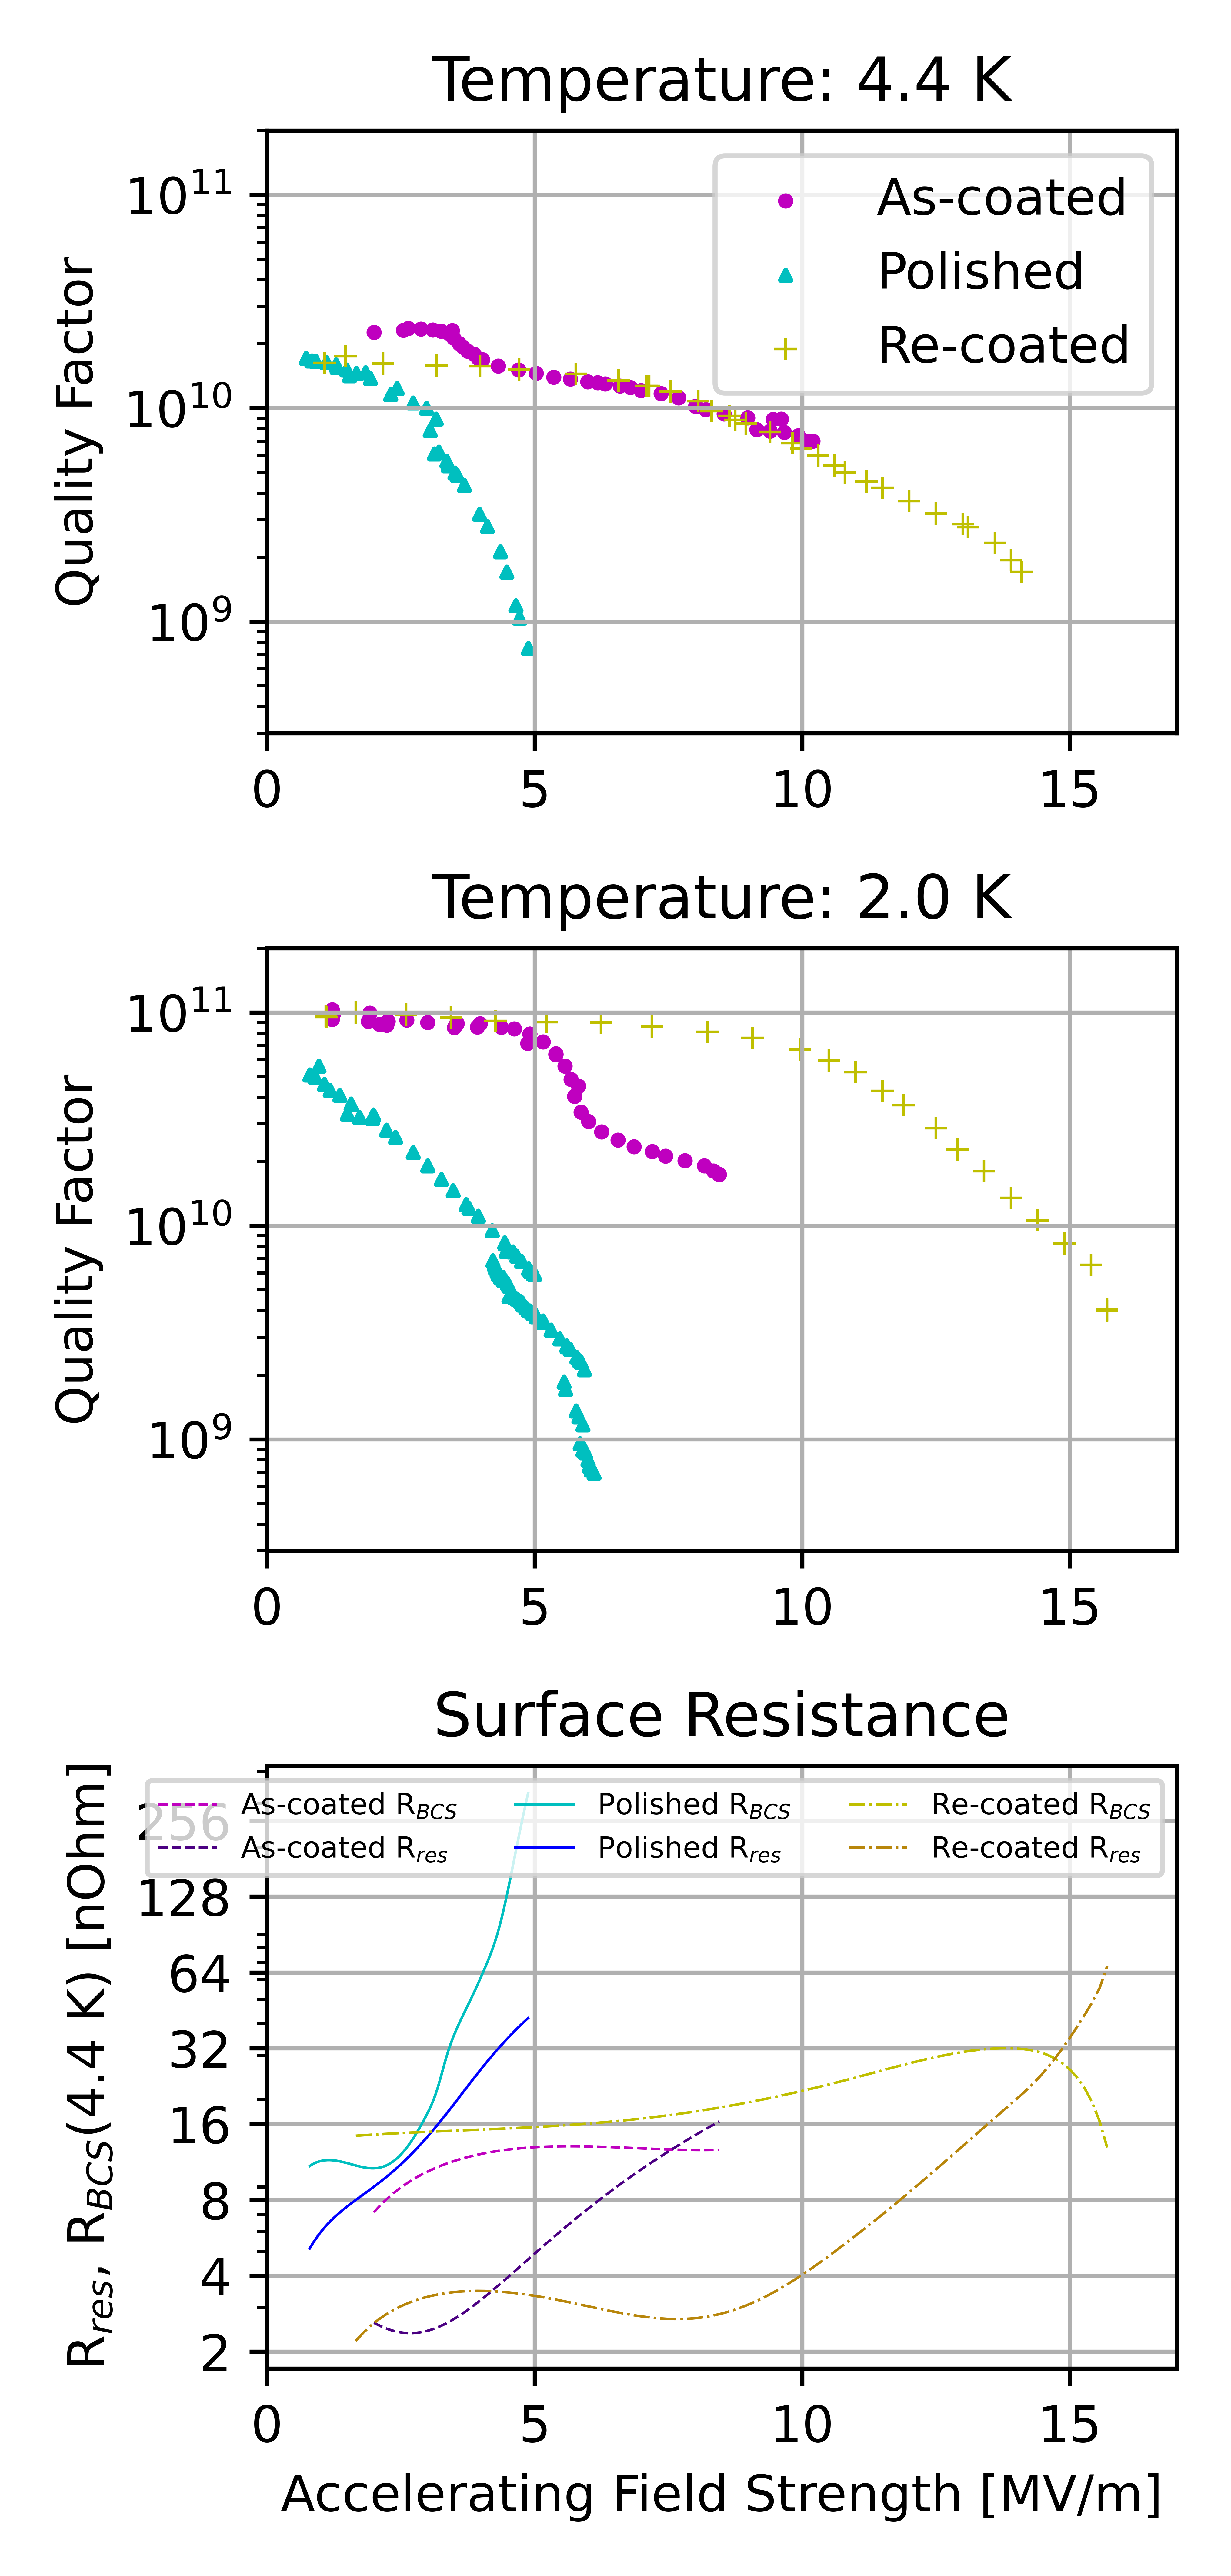
\includegraphics[width=0.8\columnwidth]{../doc/figs/VTS_Test_Graph.png}%
\caption{The RF performance of the Nb\textsubscript{3}Sn-coated SRF cavity before and after mechanically polished and after a recoating treatment. The residual resistance of the cavity is calculated from the 2.0~K measurements under the assumption that the BCS resistance is negligible at this temperature. We assume that the additional resistance measured at 4.4~K is entirely BCS resistance. These assumptions may be false if there are multiple Nb\textsubscript{3}Sn phases on the surface.}%
\label{fig:vtstestgraph}%
\end{figure}

%
\section{Discussion}%
\label{sec:Discussion}%
Using mechanical polishing, we are able to produce smooth Nb\textsubscript{3}Sn films with surface roughness less than 20~nm. This level of surface roughness has thus far been impossible to achieve using existing methods.\cite{posen2021advances,pudasaini2018studies,pudasaini2017post,hu2019reducing} We have also shown that this smoothing can be achieved with only a few hundred nanometers of material removal, much less than what would be required for chemical polishing methods.

This study also shows that mechanical polishing can be used to improve the performance of Nb\textsubscript{3}Sn cavities when used in conjunction with a recoating procedure. There are several reasons why polishing a Nb\textsubscript{3}Sn might lead to performance improvements. The most obvious is the reduction in surface roughness, which reduces the field enhancement factor around sharp edges. This should lead to a decrease in Q-slope and an increase in quench field\cite{knobloch1999high, xu2016simulation} due to a reduction in the volume of normal conducting material interacting with the RF field. However, only one of these effects is experimentally measured, the increase in quench field, while the Q-slope remains mostly unchanged.

Another effect of polishing is a reduction in the film thickness. Nb\textsubscript{3}Sn is a poor thermal conductor compared to Nb, which can lead to a buildup of heat on the cavity surface. Higher surface temperatures lower the super heating critical magnetic field and increases BCS resistance causing a premature quench. By decreasing the film thickness, the thermal properties are improved which could lead to a higher quench field\cite{kulyavtsev2021simulations}. From our sample experiments we measured a removal of approximately 700~nm after 4~hours of polishing. Assuming a 3~\unit{\micro\metre} starting thickness and one dimensional heat diffusion through the film, this reduction could lead to a 30\% increase in the maximum heat flux. This effect is more significant if there is a point source of heat on the surface caused by a defect\cite{porter2021advancing}. In this case, the quench field is determined by the thermal stability of the defect. A reduction in film thickness can lead to better thermal stability and allow the cavity to reach higher gradients.

The immediate effect of polishing reduces the quality factor and accelerating gradient of the cavity despite improving the surface finish and decreasing film thickness. The exact cause of this performance degradation is not known. There are two types of defects that could cause a degradation in performance; pre-existing subsurface defects that were created during the initial coating of the cavity and defects that were created by the tumbling process.

Pre-existing defects existing below the surface of the as coated film such as tin-depleted regions\cite{lee2018atomic} and other poorly conducting Nb\textsubscript{3}Sn phases are known to exist below the surface of the film and could be exposed to the surface by the removal of material through polishing. In a previous study, we have shown that tin-depleted regions and regions where the film becomes very thin are common in tin vapor-diffusion coated samples near the surface were they could be exposed by the polishing process\cite{10073616}. 

Another possible cause for performance degradation is surface damage or other defects caused by the polishing process. Residual abrasive particles can be seen in the SEM images of the polished samples. Cleaning the surface removes most of the contamination, but there may still be some abrasive particles left on the surface, which could cause performance degradation. Surface damage such as cracks or scratches on the film could also degrade performance, although this seems unlikely as no surface damage was detected on the Nb\textsubscript{3}Sn samples polished with felt cubes. It is also possible that the oxide that forms on the Nb\textsubscript{3}Sn surface after polishing is unfavorable for performance compared to the oxide that forms in the furnace after the coating process.

After the recoating process was applied, the cavity performance was improved over the unpolished state. We theorize that the re-coating procedure can eliminate both of the aforementioned defect types. A short, low-temperature coating is sufficient to diffuse more Sn into any exposed tin-depleted regions that may have been exposed during the polishing. It is also possible that the Sn vapor can diffuse into and repair any small cracks that may have been created during tumbling. Also, by raising the temperature of the Nb\textsubscript{3}Sn, the surface oxide layer created during the tumbling is dissolved, and a new surface oxide is created when the cavity is exposed to air. Only the residual alumina particles are unaffected by the recoating, since they are thermally stable at 1000~\unit{\celsius}. However, it is difficult to determine the exact effects of the recoating without performing a thorough cutout analysis on the cavity. Further studies are under way to determine the cause of the performance degradation after mechanical polishing and the effects of the recoating procedure on the Nb\textsubscript{3}Sn surface.

It is also worth studying the recoating process on its own to determine if there is any effect on unpolished cavities. The extra Sn provided by the recoating could improve the stoichiometry of the surface and eliminate tin-deficient regions. Additionally, the effects of annealing the cavity at 1000~\unit{\celsius} could also be causing a performance increase.

Even after polishing and recoating, the accelerating gradient of the mechanically polished cavity is still below that of the current record holding cavity\cite{posen2021advances}. This suggests that there are multiple mechanisms that contribute towards cavity quench with surface roughness being one of them. By using mechanical polishing to eliminate the effects of surface roughness on the cavity performance, we can isolate these other mechanisms. We plan to apply mechanical polishing to Nb\textsubscript{3}Sn cavities with better as-coated performance. If the performance improvement shown in this paper can be realized in cavities with better initial performance, we could see a drastic increase in the maximum accelerating gradient.

Utilizing CBP for Nb\textsubscript{3}Sn SRF cavities is still an under-explored process, and the research presented in this paper only shows our initial attempts at optimizing the process. At the moment we have only a single cavity to base our results on, which limits our ability to understand the process. There are many parameters that can be tweaked to potentially improve the cavity performance, and many questions that are left unanswered. Therefore, we must polish more cavities to understand the effects of each step of the process on the final performance.

We still do not know the effect residual abrasive particles have on the cavity performance. The alumina abrasive is not expected to contribute any significant resistive losses, but could contribute dielectric losses. The combination of ultrasonic cleaning and HPR shown in this study is likely not sufficient to entirely remove residual abrasives. Further research is necessary to find a reliable cleaning method for polished cavities. Chemical cleaning methods such as HF rinsing may be promising in this regard. Further polishing could help prevent alumina from sticking to the surface by removing crevices that alumina can gather in.

Another step that must be studied further is the recoating. The temperature, duration, and amount of Sn used are chosen to minimize any surface roughness caused by the recoating due to thermal etching mechanisms and also to prevent the growth of an excessively thick film which could negatively impact the thermal characteristics of the cavity. However, it is unclear how prominent thermal etching is or what other impact these parameters have on the film microstructure. Work still needs to be done to determine the optimum parameters for repairing the damage caused by the polishing while also minimizing any thermal etching and negative side effects. It is also worth investigating the effects of the recoating on unpolished cavities to see if any performance improvements can be made by introducing more Sn at a lower temperature after the initial coating is complete.

The ability to smooth the surface of the Nb\textsubscript{3}Sn cavities also opens opportunities to experiment with coatings of different thicknesses and grain structure which can then be polished to achieve a smoother surface than is currently possible. Having precise control of the coating thickness as well as the removal rate of the polishing step could allow for much thinner and smoother films with better thermal conduction properties. Future research should incorporate Nb\textsubscript{3}Sn coatings with different initial thicknesses.

%
\section{Conclusion}%
\label{sec:Conclusion}%
The work presented in this paper shows that centrifugal barrel polishing is a promising treatment for Nb\textsubscript{3}Sn cavities. Through a series of sample studies, we were able to develop a mechanical polishing procedure that can produce surface roughness that was previously unobtainable. We have found that it is possible to attain films with a surface roughness of 20~nm or lower. 

Furthermore, we have shown that this surface polishing technique can be used to improve the performance of Nb\textsubscript{3}Sn coated cavities when it is paired with a recoating step, which consists of a short, low-temperature Sn coating.

We also stress the fact that centrifugal barrel polishing is still a highly unexplored process for Nb\textsubscript{3}Sn SRF cavities. More research is needed to find the optimum parameters for improving cavity performance.

\section{Acknowledgements}
\label{sec:acknowledgements}
This manuscript has been authored by Fermi Research Alliance, LLC under Contract No. DE-AC02-07CH11359 with the U.S. Department of Energy, Office of Science, Office of High Energy Physics.

This work made use of the EPIC facility of Northwestern University’s NUANCE Center, which has received support from the SHyNE Resource (NSF ECCS-2025633), the IIN, and Northwestern's MRSEC program (NSF DMR-1720139).

%
\bibliography{bib}%
\end{document}